\documentclass{jknotes}
\usepackage{../joshkirklin}

\setmathfont{Latin Modern Math}
\setmathfont{GFS NeoHellenic Math}[range=bfsfup/{greek,Greek}->it]
\setmathfont{GFS NeoHellenic Math}[range=sfup/{latin,Latin}->it]

\usetikzlibrary{shapes.misc}

\tikzset{cross/.style={cross out, draw=black, minimum
size=2*(#1-\pgflinewidth), inner sep=0pt, outer sep=0pt}}
%default radius will be 1pt. 

\newcommand{\myol}[2][3]{{}\mkern#1mu\overline{\mkern-#1mu#2}}

\begin{document}

\institution{Cambridge Part III Maths}
\title{Fluid Dynamics of Environment}
\lecturer{Dr. Stuart Dalziel}
\notetaker{Charles Powell}
\date{Lent 2020}

\maketitle
\suggestionsspiel
\tableofcontents

\lecture{22/01/21}
\section{Internal waves}

\subsection{Intuitive version}

\begin{center}
	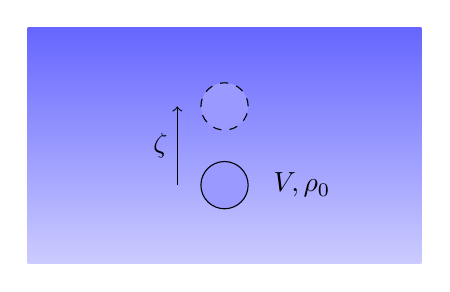
\begin{tikzpicture}
		\draw[draw=none,top color = blue!60, bottom color = blue!20] (0,0) rectangle (5, 3);
		\draw[fill=blue!40] (2.5, 1) circle (0.3);
		\draw (3, 1) node[right] {$V, \rho_0$};
		\draw[dashed,fill=blue!40] (2.5, 2) circle (0.3);
		\draw[->] (1.9, 1) -- (1.9, 2) node[midway,left] {$\zeta$};
	\end{tikzpicture}
\end{center}
Consider a fluid parcel of volume $V$ and density $\rho_0$ in a fluid with
density profile $\hat{\rho}(z)$.  Suppose the parcel is moved upwards by
$\zeta$. The parcel experiences a \emph{buoyancy force} $B = g V \zeta
\frac{\diffd \hat{\rho}}{\diffd z}$. Newton's second law gives
\begin{equation}
	\ddot{\zeta} + \left(-\frac{g}{\rho_0} \frac{\diffd \hat{\rho}}{\diffd
	z}\right) \zeta = 0
\end{equation}
The \emph{buoyancy frequency} (or Brunt-V\"{a}is\"{a}l\"{a} frequency) is
defined as 
\begin{equation}
	N^2 = - \frac{g}{\rho} \frac{\diffd \hat{\rho}}{\diffd z}
\end{equation}
which has general solution
\begin{equation}
	\zeta = A \cos N t + B \sin N t
\end{equation}
If we instead consider a fluid slab inclined at angle $\theta$ with the
vertical rather than a fluid parcel, the slab can fall in its plane much more
easily than in the vertical. Hence in this situation we have
\begin{equation}
	\ddot{\zeta} + N^2 \cos^2\theta \zeta = 0
\end{equation}
The dispersion relation is thus $\omega/N = \cos \theta$.

Now consider a sphere oscillating at frequency $\omega$ in the vertical in a
stratified fluid with density $\rho(z)$. The fluid resonates in bands at angle
$\theta$ satisfying the dispersion relation, provided $\omega < N$.
Intuitively, the group velocity must be out of the beams as energy is radiated
away.
\begin{center}
	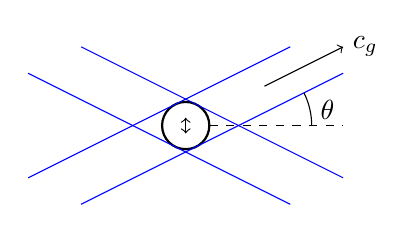
\begin{tikzpicture}
		\draw[thick] (0,0) circle (0.3);
		\draw[<->] (0, 0.1) -- (0, -0.1);
		\draw[blue] (1.328,1) -- (-2, -0.664);
		\draw[blue] (-1.328,-1) -- (2, 0.664);
		\draw[blue] (-1.328,1) -- (2, -0.664);
		\draw[blue] (1.328,-1) -- (-2, 0.664);
		\draw[dashed] (0.3, 0) -- (2, 0);
		\draw (1.6,0) arc (0:26.5:1.6-0.672);
		\draw (1.8, 0.2) node {$\theta$};
		\draw[->] (1, 0.5) -- (2,1) node[right] {$\symbf{c}_g$};
	\end{tikzpicture}
\end{center}

At the leading edge of the rays, baroclinic vorticity is generated by the
movement of fluid of different density to its surroundings. This provides the
mechanism for the instability.

\subsection{Rigorous derivation}
Consider a fluid in which the mean pressure $p_0(z)$ and the mean density
$\rho_0(z)$ are in hydrostatic balance when the fluid is at rest:
\begin{equation}
	\frac{\diffd p_0}{\diffd z} = - \rho_0 g
\end{equation}

Assume that the vertical lengthscale for $\rho_0$ variation is $L$. Motion is
governed by the Navier-Stokes equations \eqref{eq:incomp} and \eqref{eq:ns} with
$\nu = 0$, and mass conservation \eqref{eq:masscons}. 
\begin{align}
	\nabla \cdot \symbf{u} &= 0 \label{eq:incomp} \\
	\rho \frac{\partial \symbf{u}}{\partial t} + \rho
	(\symbf{u}\cdot\nabla)\symbf{u} &= - \nabla p - \rho g \hat{\symbf{z}}
	\label{eq:ns} \\
	\left(\frac{\partial}{\partial t} + \symbf{u}\cdot \nabla \right) \rho = 0
	\label{eq:masscons}
\end{align}

Following the Boussinesq approximation, assume small perturbations to the mean
state: $\rho = \rho_0(z) + \tilde{\rho}$ and $p = p_0(z) + \tilde{p}$ where
$\tilde{p} \ll p_0, \tilde{\rho} \ll \rho_0$. Under this approximation, the
momentum equation \eqref{eq:ns} becomes
\begin{align}
	\frac{\partial \symbf{u}}{\partial t} + (\symbf{u}\cdot\nabla)\symbf{u} 
	&= - \frac{1}{\rho_0}\nabla p - \frac{\rho}{\rho_0} g \hat{\symbf{z}} \\ 
	&= - \frac{1}{\rho_0} \nabla(p + \rho_0 g z) - g' \hat{\symbf{z}}
\end{align}
where $g' = g(\rho-\rho_0)/\rho_0$ is the \emph{reduced gravity}. We now
linearise $\symbf{u}$ about a state of rest, ignoring second order quantities
in the velocity disturbance $\symbf{u}'$. It is now further desirable to split
the disturbance components into $\tilde{\rho} = \hat{\rho} + \rho', \tilde{p}
= \hat{p} + p'$ where $\hat{\rho}, \hat{p}$ are in hydrostatic balance. We
have
\begin{align}
	\nabla \cdot \symbf{u}' &= 0  \\
	\frac{\partial \rho'}{\partial t} + w' \frac{\diffd \hat{\rho}}{\diffd z}
							&= \frac{\partial \rho'}{\partial t} - w' \frac{\rho_0}{g}N^2 
							= 0 \\
	\frac{\partial \symbf{u}'}{\partial t} 
							&= -\frac{1}{\rho_0}\nabla (p_0+\hat{p}) -
							\frac{g\hat{\rho}}{\rho_0}\hat{\symbf{z}} -
							\frac{1}{\rho_0} \nabla p' -
							\frac{g\rho'}{\rho_0}\hat{\symbf{z}}
							\label{eq:idk} 
\end{align}
Hydrostatic balance eliminates the first two RHS terms of the momentum
equation; the
hydrostatic pressure field is 
\begin{equation}
	p_0 + \hat{p} = -\int g \hat{\rho} \, \diffd z
\end{equation}
Finally we have
\begin{equation}
	\frac{\partial \symbf{u}'}{\partial t} = -\frac{1}{\rho_0} \nabla p' -
	\frac{g\rho'}{\rho_0} \hat{\symbf{z}}
\end{equation}
Define buoyancy $b = - g \rho'/\rho_0$. The governing equations are now
\begin{align}
	\frac{\partial b}{\partial t} &= -\frac{1}{\rho_0} \nabla p' + b
	\hat{\symbf{z}} \\
	\frac{\partial \symbf{u}'}{\partial t} &= -\frac{1}{\rho_0} \nabla p' + b
	\hat{\symbf{z}}
\end{align}
To eliminate pressure, we take the curl of the momentum equation to get
\begin{equation}
	\frac{\partial \symbf{\zeta}'}{\partial t} = -\hat{\symbf{z}}\times\nabla
	b
\end{equation}
where $\symbf{\zeta}' = \nabla \times \symbf{u}'$ is the disturbance
vorticity. Using the buoyancy equation we have
\begin{equation}
	\left[ \nabla^2 \frac{\partial^2}{\partial t^2} + N^2 \nabla_H^2\right] w'
	= 0
\end{equation}
where $\nabla_H = (\partial_x,\partial_y)$ is the horizontal gradient
operator. This equation admits plane wave solutions
\begin{equation}
	w'(\symbf{x},t) = \Re\left[ \hat{w}(t) e^{i(k_x x + k_y y - \omega
	t)}\right]
\end{equation}
where $\hat{w}$ satisfies
\begin{equation}
	\frac{\diffd^2 \hat{w}}{\diffd z^2} + (k_x^2 + k_y^2)(\frac{N^2}{\omega^2}
	- 1) \hat{w} = 0
\end{equation}
which has general solution
\begin{align}
	\hat{w} &= \Re\left[ A e^{-inz} + Be^{inz}\right] \\
	n^2 &= (k_x^2 + k_y^2)(\frac{N^2}{\omega^2} - 1)
\end{align}
If $\omega > N$, $n$ is imaginary and, defining $\gamma =
\sqrt{1-N^2/\omega^2}$, we have
\begin{equation}
	w' = (A e^{-\gamma k z} + B e^{\gamma kz}) e^{i(k_x x + k_y y - \omega
	t)}
\end{equation}
When $N = 0$, we get potential flow. If $0 < N < \omega$ then we have rescaled
potential flow, with scaling $\gamma$. If $\omega < N$ then $n$ is real and
solutions are oscillatory with
\begin{equation}
	n^2 = k z^2 = (k_x^2 + k_y^2)(\frac{N^2}{\omega^2} - 1)
\end{equation}
The wavenumber vector is $\symbf{k} = (k_x, k_y, k_z) = (k,l,m)$. Hence
\begin{equation}
	\frac{\omega^2}{N^2} = \frac{k_x^2 + k_y^2}{k_x^2+k_y^2+k_z^2} = 1 -
	\frac{k_z^2}{\abs{\symbf{k}}^2} = \cos^2 \theta
\end{equation}
where $\theta$ is the angle between $\symbf{k}$ and the horizontal plane.

\end{document}

